% Options for packages loaded elsewhere
\PassOptionsToPackage{unicode}{hyperref}
\PassOptionsToPackage{hyphens}{url}
\PassOptionsToPackage{dvipsnames,svgnames,x11names}{xcolor}
%
\documentclass[
  12pt,
]{article}

\usepackage{amsmath,amssymb}
\usepackage{iftex}
\ifPDFTeX
  \usepackage[T1]{fontenc}
  \usepackage[utf8]{inputenc}
  \usepackage{textcomp} % provide euro and other symbols
\else % if luatex or xetex
  \usepackage{unicode-math}
  \defaultfontfeatures{Scale=MatchLowercase}
  \defaultfontfeatures[\rmfamily]{Ligatures=TeX,Scale=1}
\fi
\usepackage{lmodern}
\ifPDFTeX\else  
    % xetex/luatex font selection
\fi
% Use upquote if available, for straight quotes in verbatim environments
\IfFileExists{upquote.sty}{\usepackage{upquote}}{}
\IfFileExists{microtype.sty}{% use microtype if available
  \usepackage[]{microtype}
  \UseMicrotypeSet[protrusion]{basicmath} % disable protrusion for tt fonts
}{}
\makeatletter
\@ifundefined{KOMAClassName}{% if non-KOMA class
  \IfFileExists{parskip.sty}{%
    \usepackage{parskip}
  }{% else
    \setlength{\parindent}{0pt}
    \setlength{\parskip}{6pt plus 2pt minus 1pt}}
}{% if KOMA class
  \KOMAoptions{parskip=half}}
\makeatother
\usepackage{xcolor}
\usepackage[top=1in,bottom=1in,left=1in,right=1in]{geometry}
\setlength{\emergencystretch}{3em} % prevent overfull lines
\setcounter{secnumdepth}{5}
% Make \paragraph and \subparagraph free-standing
\makeatletter
\ifx\paragraph\undefined\else
  \let\oldparagraph\paragraph
  \renewcommand{\paragraph}{
    \@ifstar
      \xxxParagraphStar
      \xxxParagraphNoStar
  }
  \newcommand{\xxxParagraphStar}[1]{\oldparagraph*{#1}\mbox{}}
  \newcommand{\xxxParagraphNoStar}[1]{\oldparagraph{#1}\mbox{}}
\fi
\ifx\subparagraph\undefined\else
  \let\oldsubparagraph\subparagraph
  \renewcommand{\subparagraph}{
    \@ifstar
      \xxxSubParagraphStar
      \xxxSubParagraphNoStar
  }
  \newcommand{\xxxSubParagraphStar}[1]{\oldsubparagraph*{#1}\mbox{}}
  \newcommand{\xxxSubParagraphNoStar}[1]{\oldsubparagraph{#1}\mbox{}}
\fi
\makeatother

\usepackage{color}
\usepackage{fancyvrb}
\newcommand{\VerbBar}{|}
\newcommand{\VERB}{\Verb[commandchars=\\\{\}]}
\DefineVerbatimEnvironment{Highlighting}{Verbatim}{commandchars=\\\{\}}
% Add ',fontsize=\small' for more characters per line
\usepackage{framed}
\definecolor{shadecolor}{RGB}{241,243,245}
\newenvironment{Shaded}{\begin{snugshade}}{\end{snugshade}}
\newcommand{\AlertTok}[1]{\textcolor[rgb]{0.68,0.00,0.00}{#1}}
\newcommand{\AnnotationTok}[1]{\textcolor[rgb]{0.37,0.37,0.37}{#1}}
\newcommand{\AttributeTok}[1]{\textcolor[rgb]{0.40,0.45,0.13}{#1}}
\newcommand{\BaseNTok}[1]{\textcolor[rgb]{0.68,0.00,0.00}{#1}}
\newcommand{\BuiltInTok}[1]{\textcolor[rgb]{0.00,0.23,0.31}{#1}}
\newcommand{\CharTok}[1]{\textcolor[rgb]{0.13,0.47,0.30}{#1}}
\newcommand{\CommentTok}[1]{\textcolor[rgb]{0.37,0.37,0.37}{#1}}
\newcommand{\CommentVarTok}[1]{\textcolor[rgb]{0.37,0.37,0.37}{\textit{#1}}}
\newcommand{\ConstantTok}[1]{\textcolor[rgb]{0.56,0.35,0.01}{#1}}
\newcommand{\ControlFlowTok}[1]{\textcolor[rgb]{0.00,0.23,0.31}{\textbf{#1}}}
\newcommand{\DataTypeTok}[1]{\textcolor[rgb]{0.68,0.00,0.00}{#1}}
\newcommand{\DecValTok}[1]{\textcolor[rgb]{0.68,0.00,0.00}{#1}}
\newcommand{\DocumentationTok}[1]{\textcolor[rgb]{0.37,0.37,0.37}{\textit{#1}}}
\newcommand{\ErrorTok}[1]{\textcolor[rgb]{0.68,0.00,0.00}{#1}}
\newcommand{\ExtensionTok}[1]{\textcolor[rgb]{0.00,0.23,0.31}{#1}}
\newcommand{\FloatTok}[1]{\textcolor[rgb]{0.68,0.00,0.00}{#1}}
\newcommand{\FunctionTok}[1]{\textcolor[rgb]{0.28,0.35,0.67}{#1}}
\newcommand{\ImportTok}[1]{\textcolor[rgb]{0.00,0.46,0.62}{#1}}
\newcommand{\InformationTok}[1]{\textcolor[rgb]{0.37,0.37,0.37}{#1}}
\newcommand{\KeywordTok}[1]{\textcolor[rgb]{0.00,0.23,0.31}{\textbf{#1}}}
\newcommand{\NormalTok}[1]{\textcolor[rgb]{0.00,0.23,0.31}{#1}}
\newcommand{\OperatorTok}[1]{\textcolor[rgb]{0.37,0.37,0.37}{#1}}
\newcommand{\OtherTok}[1]{\textcolor[rgb]{0.00,0.23,0.31}{#1}}
\newcommand{\PreprocessorTok}[1]{\textcolor[rgb]{0.68,0.00,0.00}{#1}}
\newcommand{\RegionMarkerTok}[1]{\textcolor[rgb]{0.00,0.23,0.31}{#1}}
\newcommand{\SpecialCharTok}[1]{\textcolor[rgb]{0.37,0.37,0.37}{#1}}
\newcommand{\SpecialStringTok}[1]{\textcolor[rgb]{0.13,0.47,0.30}{#1}}
\newcommand{\StringTok}[1]{\textcolor[rgb]{0.13,0.47,0.30}{#1}}
\newcommand{\VariableTok}[1]{\textcolor[rgb]{0.07,0.07,0.07}{#1}}
\newcommand{\VerbatimStringTok}[1]{\textcolor[rgb]{0.13,0.47,0.30}{#1}}
\newcommand{\WarningTok}[1]{\textcolor[rgb]{0.37,0.37,0.37}{\textit{#1}}}

\providecommand{\tightlist}{%
  \setlength{\itemsep}{0pt}\setlength{\parskip}{0pt}}\usepackage{longtable,booktabs,array}
\usepackage{calc} % for calculating minipage widths
% Correct order of tables after \paragraph or \subparagraph
\usepackage{etoolbox}
\makeatletter
\patchcmd\longtable{\par}{\if@noskipsec\mbox{}\fi\par}{}{}
\makeatother
% Allow footnotes in longtable head/foot
\IfFileExists{footnotehyper.sty}{\usepackage{footnotehyper}}{\usepackage{footnote}}
\makesavenoteenv{longtable}
\usepackage{graphicx}
\makeatletter
\def\maxwidth{\ifdim\Gin@nat@width>\linewidth\linewidth\else\Gin@nat@width\fi}
\def\maxheight{\ifdim\Gin@nat@height>\textheight\textheight\else\Gin@nat@height\fi}
\makeatother
% Scale images if necessary, so that they will not overflow the page
% margins by default, and it is still possible to overwrite the defaults
% using explicit options in \includegraphics[width, height, ...]{}
\setkeys{Gin}{width=\maxwidth,height=\maxheight,keepaspectratio}
% Set default figure placement to htbp
\makeatletter
\def\fps@figure{htbp}
\makeatother

\usepackage{booktabs}
\usepackage{longtable}
\usepackage{array}
\usepackage{multirow}
\usepackage{wrapfig}
\usepackage{float}
\usepackage{colortbl}
\usepackage{pdflscape}
\usepackage{tabu}
\usepackage{threeparttable}
\usepackage{threeparttablex}
\usepackage[normalem]{ulem}
\usepackage{makecell}
\usepackage{xcolor}
\usepackage{amsmath,amssymb}
\usepackage{booktabs}
\usepackage{threeparttable}
\usepackage{setspace}
\doublespacing
\makeatletter
\@ifpackageloaded{caption}{}{\usepackage{caption}}
\AtBeginDocument{%
\ifdefined\contentsname
  \renewcommand*\contentsname{Table of contents}
\else
  \newcommand\contentsname{Table of contents}
\fi
\ifdefined\listfigurename
  \renewcommand*\listfigurename{List of Figures}
\else
  \newcommand\listfigurename{List of Figures}
\fi
\ifdefined\listtablename
  \renewcommand*\listtablename{List of Tables}
\else
  \newcommand\listtablename{List of Tables}
\fi
\ifdefined\figurename
  \renewcommand*\figurename{Figure}
\else
  \newcommand\figurename{Figure}
\fi
\ifdefined\tablename
  \renewcommand*\tablename{Table}
\else
  \newcommand\tablename{Table}
\fi
}
\@ifpackageloaded{float}{}{\usepackage{float}}
\floatstyle{ruled}
\@ifundefined{c@chapter}{\newfloat{codelisting}{h}{lop}}{\newfloat{codelisting}{h}{lop}[chapter]}
\floatname{codelisting}{Listing}
\newcommand*\listoflistings{\listof{codelisting}{List of Listings}}
\makeatother
\makeatletter
\makeatother
\makeatletter
\@ifpackageloaded{caption}{}{\usepackage{caption}}
\@ifpackageloaded{subcaption}{}{\usepackage{subcaption}}
\makeatother

\ifLuaTeX
  \usepackage{selnolig}  % disable illegal ligatures
\fi
\usepackage{bookmark}

\IfFileExists{xurl.sty}{\usepackage{xurl}}{} % add URL line breaks if available
\urlstyle{same} % disable monospaced font for URLs
\hypersetup{
  pdftitle={Player Market Value in Elite European Football},
  pdfauthor={Kevin Linares; Jianing Zou; Namit Shrivastava; Sagnik Chakravarti},
  colorlinks=true,
  linkcolor={blue},
  filecolor={Maroon},
  citecolor={Blue},
  urlcolor={Blue},
  pdfcreator={LaTeX via pandoc}}


\title{Player Market Value in Elite European Football}
\author{Kevin Linares \and Jianing Zou \and Namit
Shrivastava \and Sagnik Chakravarti}
\date{}

\begin{document}
\maketitle


\section{Introduction}\label{introduction}

The European football transfer market has evolved from a subjective
scouting exercise into a global financial industry exceeding €7 billion
annually. For this study, we operationalize market value using
crowd-sourced estimates from Transfermarkt, a metric widely validated in
sports economics as a robust proxy for actual transfer fees (Herm et
al., 2014). While foundational research identifies performance metrics
like goals as primary drivers (Frick, 2007), more recent scholarship
highlights a ``Superstar Effect'' where non-performance factors like
brand visibility magnify valuation (Franck \& Nüesch, 2012; Rosen,
1981). However, the market has recently bifurcated into a pre-2020
hyper-inflationary era, termed the ``Neymar Effect'' (Poli et al.,
2017), and a post-2020 pandemic correction (Drewes et al., 2021). This
trajectory was violently interrupted by the COVID-19 pandemic, which
caused an estimated €8.7 billion revenue shortfall across European
football (Deloitte, 2021). Existing models typically treat players as
static units nested within single clubs, ignoring the dynamic reality
where players transfer between teams and accumulate value from both
their portable human capital and the institutional prestige of their
current employer. Neglecting this cross-classified structure likely
misestimates the true drivers of market value in this volatile era. To
address these limitations, this study applies a cross-classified
multilevel model to a decade of transfer data (2013--2024), centering
the analysis at the 2020 pandemic baseline to quantify the impact of
this structural break. We attempt to disentangle individual reputation
from club context by investigate four critical dynamics:

\begin{enumerate}
\def\labelenumi{\arabic{enumi}.}
\tightlist
\item
  The non-linear ``Boom and Bust'' market trajectory. How has the
  transfer market evolved relative to the 2020 baseline? Specifically,
  does the market exhibit a non-linear ``Boom and Bust'' cycle that
  linear models miss?
\item
  The biological constraints of the player career arc. How does market
  valuation evolve across a player's biological career, and at what
  specific age does this value peak?
\item
  The valuation signal of ``Squad Status'' via relative playing time. To
  what degree does ``Squad Status''---defined by relative playing
  time---predict market value independent of raw performance output?
\item
  The existence of contextual premiums for club diversity or discounts
  for domestic talent in a globalized labor market. How does squad
  internationalization affect player market values, and do domestic
  players face a valuation penalty compared to foreign players?
\end{enumerate}

\section{Method}\label{method}

\subsection{Sample and Data}\label{sample-and-data}

We obtained data from Transfermarkt and UEFA official rankings using
purposive sampling to select the top 21 European clubs based on 10-year
averaged UEFA coefficient rankings\footnote{UEFA coefficient rankings
  are a points-based system used by European soccer's governing body to
  rank national associations and clubs based on their performance in
  European competitions, which determines qualification spots and
  seeding for tournaments like the Champions League and Europa League.}.
From these clubs we identified players who had a full season from 2013
through 2024 resulting in a sample of 7,023 player-season observations
from 2,159 unique players across. After listwise deletion of cases with
missing citizenship data (approximately 2\% loss), players averaged 26.5
years of age (\emph{SD} = 4.6). Critically, 441 players (20.4\%) played
for multiple clubs during the study period, justifying our
cross-classified modeling approach.

Our primary outcome variable is the natural logarithm of the player's
inflation-adjusted yearly average market value (in 2024 USD). Predictors
are categorized into three distinct domains: (1) Player Characteristics,
including age, height, position (Attacker, Midfielder, etc.), and
citizenship status relative to the club (homegrown vs.~foreign); (2)
performance and status, captured by goals, assists, red/yellow cards,
and playing time; and (3) club context, specifically the proportion of
foreign players on the roster and the club's UEFA coefficient, which
serves as a proxy for recent competitive success and prestige. For
further descriptive statistics on each variable see Appendix A, Table1.

\subsection{Model Specification}\label{model-specification}

Our data exhibit a cross-classified structure where players (\emph{i})
are constant units, but club membership (\emph{j}) changes over time
(\emph{t}). When a player transfers from club \(j_1\) to club \(j_2\),
club-level predictors such as internationalization and UEFA ranking that
vary by year, are updated to reflect the new club's characteristics.
Figure 1 visualizes our cross-classified design with an example from
three players.

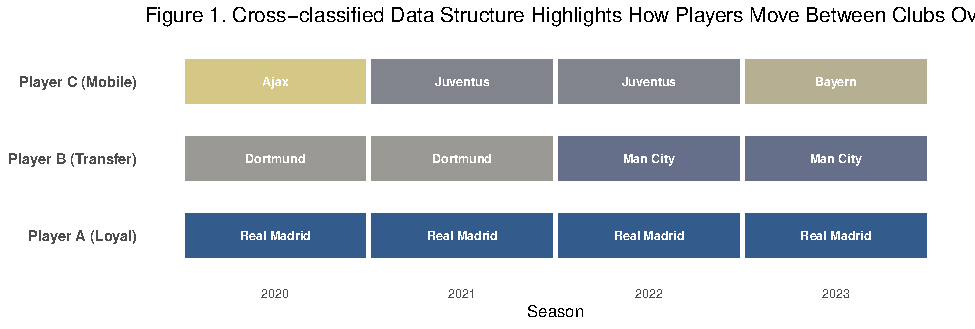
\includegraphics{Project_Paper_files/figure-pdf/unnamed-chunk-1-1.pdf}

This structure requires modeling player and club as crossed random
effects rather than nested effects. Crucially, because club attributes
like internationalization and UEFA ranking vary year-to-year, they are
modeled as Level 1 (time-varying) predictors rather than static Level 2
traits.

\textbf{Level 1: Observation Model (Time-Varying Effects)}

At the observation level, the log-transformed market value is modeled as
a function of the player-club intercept (\(\pi_{0ij}\)), algebraic time
trends, biological aging, and dynamic contextual metrics:

\[ \begin{aligned} \log(\text{MV})_{tij} &= \pi_{0ij} \\ &+ \pi_{1j}(\text{Year}_{t}) + \pi_{2j}(\text{Year}^2_{t}) + \pi_{3}(\text{Year}^3_{t}) \\ &+ \pi_{4}(\text{Age}_{it} - \bar{A}) + \pi_{5}(\text{Age}_{it} - \bar{A})^2 \\ &+ \pi_{6}(\text{Mins}_{Z,it}) \\ &+ \pi_{7}(\text{Foreign}_{tj}) + \pi_{8}(\text{UEFA}_{tj}) \\ &+ \mathbf{\Pi}_{perf} + \epsilon_{tij} \end{aligned} \]

\emph{Note: MV = Market Value. The subscripts} \({tj}\) for Foreign and
UEFA denote that these club attributes vary by time \(t\).

\[ \begin{aligned}
\boldsymbol{\Pi}_{perf}
&=
\pi_9(\text{Goals}_{tij}) 
+ \pi_{10}(\text{Assists}_{tij}) \\ &
+ \pi_{11}(\text{RedCards}_{tij}) 
+ \pi_{12}(\text{YellowCards}_{tij})\\ &
\end{aligned}\]

\textbf{Level 2a: Player Model (Time-Invariant Traits)}

The player-club intercept (\(\pi_{0ij}\)) is decomposed into a fixed
component based on static player characteristics and a random player
effect (\(u_{0i}\)):

\[ \pi_{0ij} = \beta_{0j} + \gamma_{1}(\text{Height}_{i}) + \gamma_{2}(\text{Citizen}_{ij}) + \mathbf{\Gamma}_{demog} + u_{0i} \]

\[ \begin{aligned}
\mathbf{\Gamma}_{\text{demog}}
&=
\sum_{k=1}^{K-1} \gamma_{\text{pos},k} \, 
(\text{Position}_{ik})
\;+\;
\sum_{r=1}^{R-1} \gamma_{\text{reg},r} \, (\text{Region}_{ir})
\end{aligned}\]

\textbf{Level 2b: Club Model (Contextual Trajectories)}

The club baseline (\(\beta_{0j}\)) and the time-varying slope parameters
(\(\pi_{1j}, \pi_{2j}\)) include random effects to allow for
heterogeneity in both growth velocity and trajectory curvature:

\[ \begin{aligned} \beta_{0j} &= \delta_{00} + v_{0j} \quad &\text{(Baseline Prestige)} \\ \pi_{1j} &= \delta_{10} + v_{1j} \quad &\text{(Linear Growth Deviation)} \\ \pi_{2j} &= \delta_{20} + v_{2j} \quad &\text{(Quadratic Curvature Deviation)} \\ \pi_{3} &= \delta_{30} \quad &\text{(Fixed Cubic Trend)} \end{aligned} \]

\textbf{Variance-Covariance Structure}

\[ u_{0i} \sim N(0, \sigma^2_{u}) \quad , \quad  \begin{pmatrix} v_{0j} \\ v_{1j} \\ v_{2j} \end{pmatrix} \sim N \left( \mathbf{0}, \begin{pmatrix} \sigma^2_{Int} & \sigma_{01} & \sigma_{02} \\ \sigma_{01} & \sigma^2_{Lin} & \sigma_{12} \\ \sigma_{02} & \sigma_{12} & \sigma^2_{Quad} \end{pmatrix} \right) \]

\subsection{Variables and Centering
Strategies}\label{variables-and-centering-strategies}

We apply a strategic centering and transformation strategy to isolate
the pandemic's structural impact and test non-linear market dynamics by
centering season year at the onset of COVID-19 in 2020. We include
polynomial terms to capture theorized non-linearities (Figure 2): a
cubic term for time to model the ``Boom-and-Bust'' cycle (e.g.,
pre-pandemic inflation, post-pandemic correction), and a quadratic term
for Age to test the biological ``Inverted-U'' career trajectory. Minutes
Played was standardized within each club-year to isolate player squad
status (e.g., Starter vs.~Bench) from team rotation policies, while
performance metrics were position-centered to account for role-specific
expectations.\footnote{Performance expectations vary by role: A goal
  from a striker is routine while for a defender is exceptional.
  Position-centering transforms raw counts into ``performance above
  expectation'' metrics, ensuring the model captures relative
  contributions rather than treating goals and assists equally.}

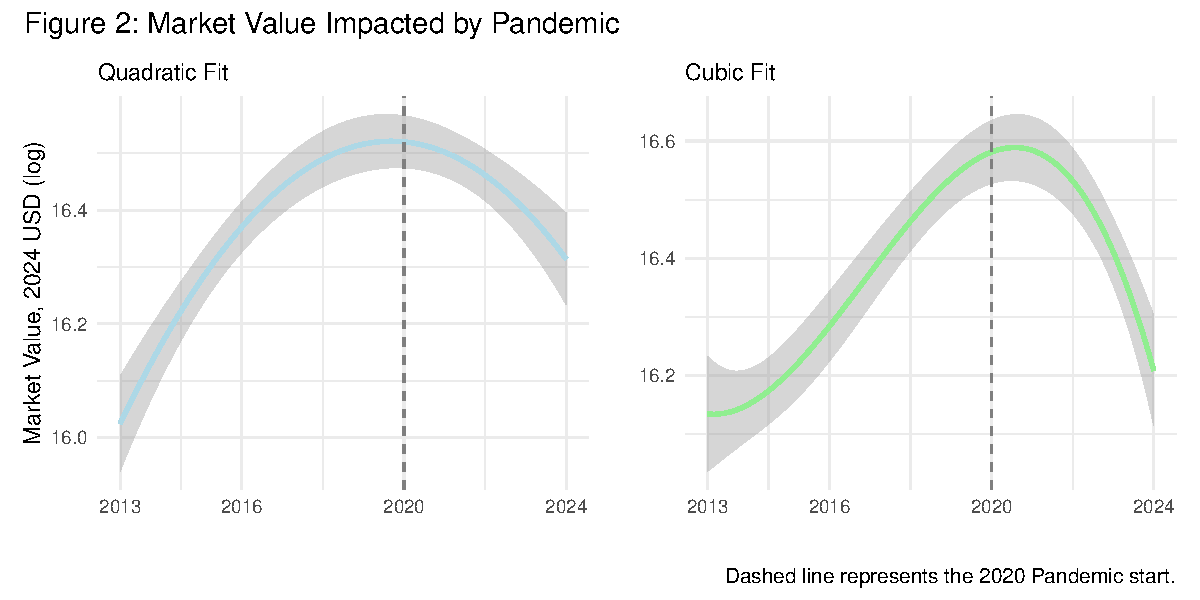
\includegraphics{Project_Paper_files/figure-pdf/unnamed-chunk-2-1.pdf}

\subsection{Model Building and Statistical
Software}\label{model-building-and-statistical-software}

We employed sequential model building: (1) null model for ICC
estimation; (2) linear time polynomial; (3) cubic time polynomial; (4)
random slope for quadratic time at club level\footnote{We excluded
  player-level random slopes due to data sparsity; a majority of players
  appear in the dataset for only one or two seasons, making it
  mathematically impossible to disentangle their individual growth
  trajectories from residual error. In contrast, the club-level data
  provides a robust longitudinal structure with continuous observations
  across the decade, allowing for the stable estimation of club-specific
  market value trajectories.}; (5) player/club-season Level 1 predictors
with quadratic age, and all code is found in Appendix B. Model selection
and comparison was guided by Likelihood Ratio Tests (LRT) to evaluate
the statistical significance of nested model improvements, and the
Akaike Information Criterion (AIC) and Bayesian Information Criterion
(BIC). Models yielding significant LRT results (p\textless.05) and lower
values on both information criteria were retained for subsequent
analysis. We describe each model in Appendix C, Table 1 alongside ICC,
AIC, and BIC values.

All analyses were conducted in R version 4.4.1 using the
\texttt{lme4\ 1.1-37} package for mixed-effects model estimation with a
Restricted Maximum Likelihood (REML) method. REML was selected to
provide unbiased estimates of the variance components by accounting for
the degrees of freedom lost when estimating fixed effects. We utilized
the BOBYQA optimizer, which handles boundary constraints more
effectively than the default Nelder-Mead optimizer, to ensure robust
model convergence given the complexity of the random effects structure.
Significance tests used Satterthwaite approximations via the
\texttt{lmerTest\ 3.1-3} package, as well as our own function to test
random slope variances in Appendix B.

\section{Results}\label{results}

The unconditional means (null) model revealed substantial clustering at
the player level. Player-level variance accounted for 78\% of the total
variance (\(ICC_{player}=.75\)), while club-level variance accounted for
5\% (\(ICC_{club}=.03\)), highlighting that persistent individual
heterogeneity dominates market valuations. Regarding temporal dynamics,
model comparisons favored a cubic fixed effect for season year over a
linear specification, \(\chi^2(2)=45.66, p<.001\). We subsequently
tested for club-specific heterogeneity in growth trajectories. A
likelihood ratio test using a 50:50 mixture of \(\chi^2_1\) and
\(\chi^2_2\) distributions\footnote{We test whether a random slope with
  quadratic season year at the club level has better fit to the data. We
  find evidence supporting the need to include these random slopes using
  a likelihood ratio test with an alternative hypothesis,
  \(H_A=\tau_{11} > 0\) since variance should be larger than 0. To test
  this hypothesis we use the likelihood ratio test (LRT) simply by
  \(-2[\text{log likelihood}_{reduced} - \text{log likelihood}_{full}]\)
  to examine the difference. This code can be found in Appendix B.}
confirmed that adding a random linear slope significantly improved model
fit compared to the random-intercept model, \(\chi^2(5)=97.13, p<.001\),
indicating that clubs differ significantly not only in their growth
rates but also in the curvature of their market value
trajectories.\footnote{While we included random linear and quadratic
  slopes, a random cubic slope was excluded due to
  over-parameterization. Estimating only 21 clubs led to singularity;
  therefore, the quadratic specification represents the maximal
  complexity supported by the data.} Consequently, our final
best-fitting model incorporates these complex random effects alongside
time-varying player and club predictors (\(\chi^2(19)=5626, p<.001\)
compared to random slopes model). Model comparisons are shown in
Appendix C, Table 1. Here we output our final model's variance
components and fixed effects.

Our final model converged successfully with no warnings. Q-Q plots
confirmed that player-level random intercepts (\(n=2,159\)) adhered well
to normality, while club-level random effects (\(n=21\)) showed minor
tail departures expected with few Level 2 units (Maas \& Hox, 2004). The
residual versus fitted values plot revealed homoscedastic variance with
no systematic patterns. Full diagnostic plots are presented in Appendix
C.

\begin{table}[H]
\centering
\caption{Estimated Variance Components for Final Model}
\centering
\fontsize{11}{13}\selectfont
\begin{tabular}[t]{>{}l|r|r}
\hline
Component & Variance & SD\\
\hline
\textbf{Player (Reputation)} & 0.9254 & 0.9620\\
\textbf{Club (Baseline Prestige)} & 0.0541 & 0.2326\\
\textbf{Club (Linear Growth)} & 0.0105 & 0.1025\\
\textbf{Club (Quadratic Curvature)} & 0.0073 & 0.0855\\
\textbf{Residual (Unexplained)} & 0.2070 & 0.4550\\
\hline
\end{tabular}
\end{table}

\begin{table}[H]
\centering
\caption{Fixed Effects Estimates from Final Model}
\centering
\fontsize{11}{13}\selectfont
\begin{threeparttable}
\begin{tabular}[t]{>{}l|r|r|r|r|l}
\hline
Predictor & β & SE & t & \% Change & \\
\hline
\textbf{Year (linear)} & 0.002 & 0.030 & 0.08 & 0.2 & \\
\textbf{Year²} & -0.270 & 0.024 & -11.05 & -23.7 & ***\\
\textbf{Year³} & -0.117 & 0.011 & -10.98 & -11.0 & ***\\
\textbf{Height} & 0.010 & 0.004 & 2.81 & 1.0 & **\\
\textbf{Defender} & -0.403 & 0.058 & -6.97 & -33.2 & ***\\
\textbf{Goalkeeper} & -1.059 & 0.095 & -11.17 & -65.3 & ***\\
\textbf{Midfielder} & -0.190 & 0.058 & -3.29 & -17.3 & **\\
\textbf{Domestic citizen} & -0.185 & 0.031 & -5.89 & -16.9 & ***\\
\textbf{Age (linear)} & 0.019 & 0.004 & 5.02 & 1.9 & ***\\
\textbf{Age²} & -0.024 & 0.000 & -63.08 & -2.4 & ***\\
\textbf{goals} & 0.005 & 0.002 & 2.36 & 0.5 & *\\
\textbf{assists} & 0.010 & 0.003 & 3.51 & 1.0 & ***\\
\textbf{Red cards} & 0.009 & 0.022 & 0.42 & 0.9 & \\
\textbf{Yellow cards} & -0.002 & 0.003 & -0.49 & -0.2 & \\
\textbf{Minutes (Z)} & 0.350 & 0.013 & 26.20 & 41.9 & ***\\
\textbf{UEFA Coefficient} & 0.000 & 0.001 & -0.39 & 0.0 & \\
\textbf{Proportion of Foreign Players} & 0.103 & 0.104 & 0.99 & 10.8 & \\
\hline
\end{tabular}
\begin{tablenotes}[para]
\item \textit{Note: } 
\item *** p < .001, ** p < .01, * p < .05
\end{tablenotes}
\end{threeparttable}
\end{table}

\subsubsection{Market Evolution}\label{market-evolution}

Using raw polynomials centered at 2020 (\(t=0\)), our model
mathematically pinpoints the moment the market froze. The linear
coefficient at the 2020 baseline is effectively zero
(\(\pi_1 = 0.00, p = 0.93\)), indicating that at the exact onset of the
pandemic, the relentless inflation of the previous decade came to a
complete halt. The significant negative quadratic (\(\pi_2 = -0.27\))
and cubic (\(\pi_3 = -0.12\)) terms confirm the transition from a
pre-2019 ``Boom'' into a structural correction. Figure 3 visualizes the
complexity of club-level market dynamics by plotting the predicted
trajectory for all clubs individually. This faceted view highlights how
clubs diverge from the global trend. The vertical position of each chart
confirms the initial hierarchy (e.g., random Intercepts), with elite
clubs like Manchester City and Bayern Munich maintaining a consistently
higher baseline than selling clubs (e.g., Sevilla, Porto). The distinct
curvature of each line, particularly around the 2020 pandemic baseline,
illustrates the significant variance in the random slopes. Clubs with
concave trajectories (e.g., Juventus, Barcelona) plateaued or declined
rapidly, confirming the risk of stagnation. Conversely, clubs with
convex trajectories (e.g., Arsenal, Liverpool) show stronger momentum,
indicating a more resilient recovery and active value generation
throughout the decade.

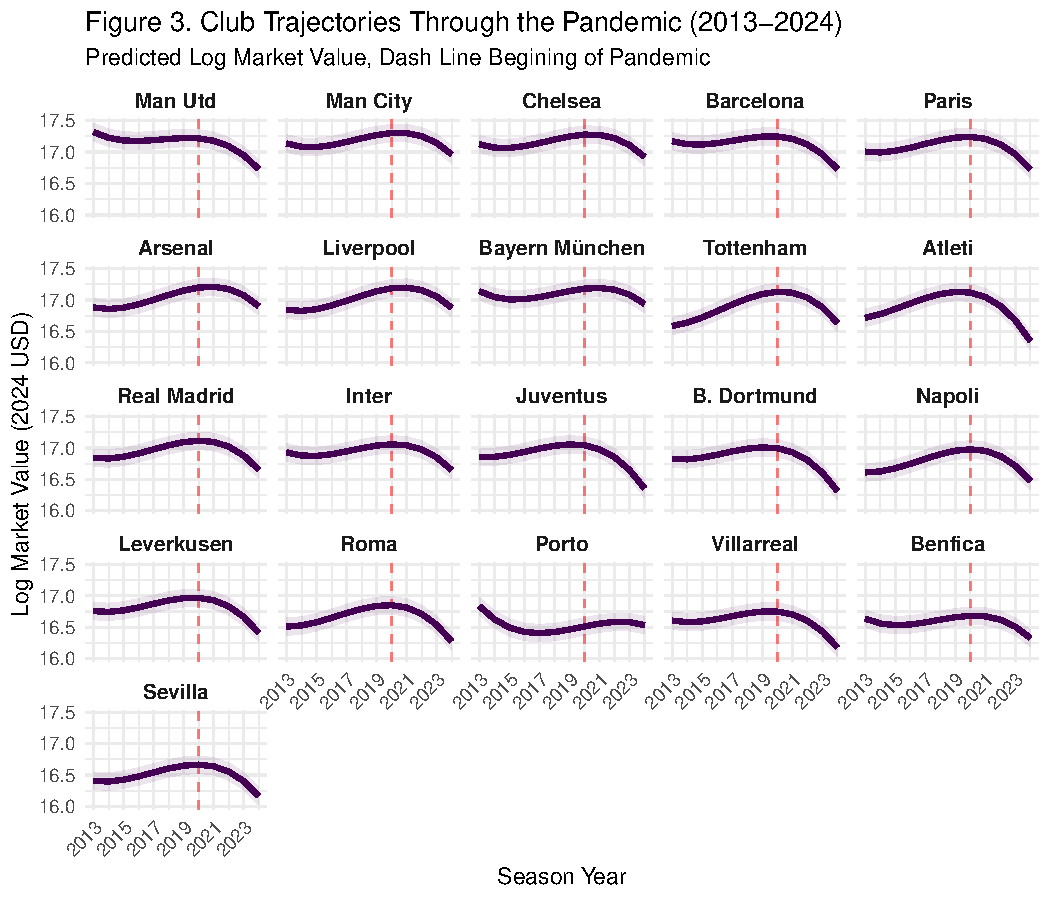
\includegraphics{Project_Paper_files/figure-pdf/unnamed-chunk-5-1.pdf}

\subsubsection{Biological Age}\label{biological-age}

Our model predicts the peak age to be 26.9\footnote{We use the delta
  method, specifically Taylor series approximation, to propagate
  uncertainty through nonlinear transformation of
  \(-\beta_{age} / (2 \times \beta_{age^2})\).} for optimal transfer
market value we visualize in Figure 4 the biological constraints on
valuation. The curve rises steeply as players transition from
`prospects' (Age 17--23), flattens into a `prime' plateau between ages
26 and 28, and declines steadily thereafter. The model predicts that a
player's value drops by approximately 1.5 log points (from a peak of
17.0 to 15.5) as they age from 27 to 35, reflecting the market's heavy
discount on older assets with limited resale potential.

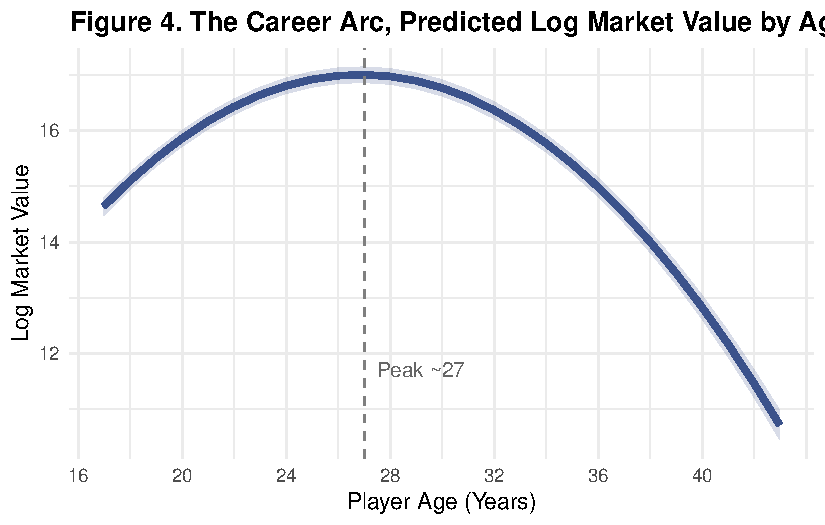
\includegraphics{Project_Paper_files/figure-pdf/unnamed-chunk-7-1.pdf}

\subsubsection{\texorpdfstring{\textbf{Contextual Premiums and
Discounts}}{Contextual Premiums and Discounts}}\label{contextual-premiums-and-discounts}

Squad status remains the dominant behavioral driver. The standardized
coefficient for minutes played (\(\pi_6 = 0.35\)) indicates a 42\%
valuation premium (\(e^{0.35}-1\)) for key starters (+1 SD) compared to
average players. Conversely, we observe a robust ``Domestic Discount,''
where homegrown citizens are valued approximately 17\% lower
(\(\gamma_2 = -0.19\)) than comparable foreign imports. While we
hypothesized a ``Diversity Premium'' for clubs with higher international
representation, the fixed effect for \texttt{foreign\_players} was
positive but not statistically significant (\(\pi_7 = 0.10, p = 0.32\))
in the final model. Similarly, the \texttt{uefa\_coefficient} showed no
significant effect (\(p = 0.70\)). This suggests that once we account
for the massive heterogeneity in Club Random Effects (i.e., Baseline
Prestige and Growth Trajectories) and individual player reputation
(\(ICC \approx 0.78\)), specific club-level metrics add little unique
explanatory power. In Figure 5, we present relative market valuation for
Level 2 fixed effects (e.g., citizenship, region origin, and position).
The coefficient for ``Homegrown (Citizen)'' falls strictly to the left
of zero, confirming that domestic players are valued significantly lower
than comparable foreign imports (\(\gamma_2=-0.19\)), potentially
reflecting the recruitment premium required to attract international
talent. Attackers (the baseline) command the highest market value. All
other positions show significant negative effects, with Goalkeepers
facing the steepest penalty (\(\gamma_{pos}=-1.06\)), suggesting the
market disproportionately rewards offensive output. While most regional
coefficients overlap with zero (indicating no difference from the
European baseline), Latin America stands out as the only region with a
positive premium (\(\gamma_{region}=0.19\)), suggesting South American
players function as a ``premium export brand'' in the global market.

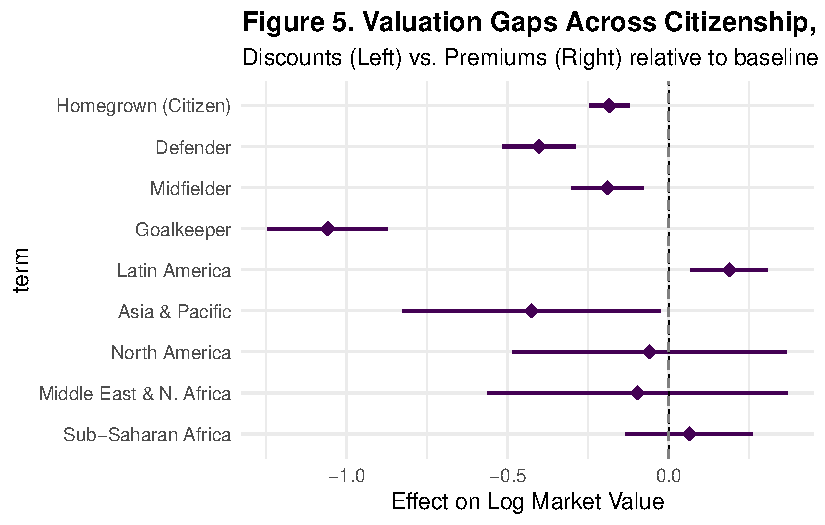
\includegraphics{Project_Paper_files/figure-pdf/unnamed-chunk-8-1.pdf}

\section{Discussion}\label{discussion}

This study demonstrates that player market value in elite football is
driven primarily by persistent individual reputation (\(ICC=0.78\)) but
is meaningfully moderated by club context and market cycles. Our
cross-classified approach properly attributes variance to portable
player effects versus transient club effects.

Centering our temporal polynomial at 2020 provides direct evidence that
the COVID-19 pandemic represented a fundamental discontinuity in the
transfer market. The near-zero linear slope at this inflection point
indicates that the decade-long inflationary trend abruptly halted,
followed by market correction. The strict inverted-U relationship
between age and market value, peaking at approximately 27 years,
confirms that transfer markets price both current ability and future
option value. The steepness of the post-peak decline (approximately 1.5
log points from age 27 to 35) reflects forward-looking assessment of
remaining productive years.

The dominance of minutes played (\(\pi_6=0.35\)) over position-specific
metrics suggests that markets rely heavily on managerial assessments as
signals of underlying quality, consistent with signaling theory. A one
standard deviation increase in relative playing time yields a 42\%
valuation premium. The finding that homegrown players are valued
approximately 17\% lower than comparable foreign imports
(\(\gamma_2=-0.19\)) suggests domestic players may be systematically
undervalued while international recruitment requires competitive bidding
that inflates prices.

In conclusion, the substantial player-level variance confirms that
persistent individual reputation dominates market assessments, while
club context creates meaningful premiums and growth trajectories. The
transfer market incorporates forward-looking assessments of biological
decline, managerial signals through squad selection, and contextual
factors that create systematic premiums and discounts. These patterns
represent both economic regularities that clubs can anticipate and
potential inefficiencies that astute market participants can exploit.

\newpage

\section*{References}\label{references}
\addcontentsline{toc}{section}{References}

Deloitte. (2021). \emph{Riding the challenge: Annual Review of Football
Finance 2021}. Deloitte Sports Business Group.
\url{https://www2.deloitte.com/uk/en/pages/sports-business-group/articles/annual-review-of-football-finance-europe.html}

Drewes, M., Daumann, F., \& Follert, F. (2021). Exploring the sports
economic impact of COVID-19 on professional soccer. \emph{Soccer \&
Society, 22}(1-2), 125-137.
\url{https://doi.org/10.1080/14660970.2020.1802256}

Herm, S., Callsen-Bracker, H. M., \& Kreis, H. (2014). When the crowd
evaluates soccer players' market values: Accuracy and evaluation
attributes of an online community. \emph{Sport Management Review,
17}(4), 484-492. \url{https://doi.org/10.1016/j.smr.2013.12.006}

Maas, C. J. M., \& Hox, J. J. (2004). Robustness issues in multilevel
regression analysis. \emph{Statistica Neerlandica, 58}(2), 127-137.
\url{https://doi.org/10.1046/j.0039-0402.2003.00252.x}

Poli, R., Ravenel, L., \& Besson, R. (2017). \emph{Transfer market
analysis} (CIES Football Observatory Monthly Report No.~27). CIES
Football Observatory.
\url{https://football-observatory.com/IMG/sites/mr/mr27/en/}

\clearpage

\newpage

\section{Appendix A}\label{appendix-a}

\subsection*{\texorpdfstring{Table 1: Variable Descriptions and
Descriptive Statistics (\emph{N}=7,168
raw)}{Table 1: Variable Descriptions and Descriptive Statistics (N=7,168 raw)}}\label{table-1-variable-descriptions-and-descriptive-statistics-n7168-raw}
\addcontentsline{toc}{subsection}{Table 1: Variable Descriptions and
Descriptive Statistics (\emph{N}=7,168 raw)}

\begin{table}[!h]
\centering\begingroup\fontsize{10}{12}\selectfont

\resizebox{\ifdim\width>\linewidth\linewidth\else\width\fi}{!}{
\begin{tabular}{>{\raggedright\arraybackslash}p{5cm}>{\raggedright\arraybackslash}p{4cm}>{\raggedright\arraybackslash}p{5cm}}
\toprule
Description & Raw Stats (Mean/SD) & Transformation Strategy\\
\midrule
\addlinespace[0.3em]
\multicolumn{3}{l}{\textbf{Continuous Variables}}\\
\hspace{1em}\textbf{Market Value (2024 USD)} & \$25.8M (29.0M) & \em{Log-transformed (ln)}\\
\hspace{1em}\textbf{Season Year} & 2018.63 (3.47) & \em{Centered at 2020 (0 = 2020)}\\
\hspace{1em}\textbf{Player Age (Years)} & 26.50 (4.58) & \em{Grand-mean centered + Quadratic}\\
\hspace{1em}\textbf{Height (cm)} & 182.10 (6.84) & \em{Grand-mean centered}\\
\hspace{1em}\textbf{Minutes Played} & 1761.77 (1337.70) & \em{Z-scored within Club-Year}\\
\hspace{1em}\textbf{Goals Scored} & 3.41 (6.25) & \em{Centered by Position Mean}\\
\hspace{1em}\textbf{Assists Made} & 2.79 (4.00) & \em{Centered by Position Mean}\\
\hspace{1em}\textbf{Club Foreign \%} & 63.5\% (11.1\%) & \em{Grand-mean centered}\\
\hspace{1em}\textbf{UEFA Coefficient} & 20.42 (6.89) & \em{Year-mean centered}\\
\hspace{1em}\textbf{Red Cards} & 0.07 (0.28) & \em{Raw count}\\
\hspace{1em}\textbf{Yellow Cards} & 3.42 (3.60) & \em{Raw count}\\
\addlinespace[0.3em]
\multicolumn{3}{l}{\textbf{Categorical Variables}}\\
\hspace{1em}\textbf{Citizenship (Homegrown)} &  & \em{Binary (1=Citizen)}\\
\hspace{1em}\textbf{- No} & 4498 (62.8\%) & \em{}\\
\hspace{1em}\textbf{- Yes} & 2567 (35.8\%) & \em{}\\
\hspace{1em}\textbf{- NA} & 103 (1.4\%) & \em{}\\
\hspace{1em}\textbf{Primary Position} &  & \em{Factor (Ref: Attack)}\\
\hspace{1em}\textbf{- Attack} & 1925 (26.9\%) & \em{}\\
\hspace{1em}\textbf{- Defender} & 2448 (34.2\%) & \em{}\\
\hspace{1em}\textbf{- Goalkeeper} & 605 (8.4\%) & \em{}\\
\hspace{1em}\textbf{- Midfield} & 2190 (30.6\%) & \em{}\\
\hspace{1em}\textbf{Region of Origin} &  & \em{Factor (Ref: Europe)}\\
\hspace{1em}\textbf{- East Asia \& Pacific} & 69 (1.0\%) & \em{}\\
\hspace{1em}\textbf{- Europe \& Central Asia} & 5139 (71.7\%) & \em{}\\
\hspace{1em}\textbf{- Latin America \& Caribbean} & 1441 (20.1\%) & \em{}\\
\hspace{1em}\textbf{- Middle East \& North Africa} & 56 (0.8\%) & \em{}\\
\hspace{1em}\textbf{- North America} & 52 (0.7\%) & \em{}\\
\hspace{1em}\textbf{- Sub-Saharan Africa} & 303 (4.2\%) & \em{}\\
\hspace{1em}\textbf{- NA} & 108 (1.5\%) & \em{}\\
\bottomrule
\end{tabular}}
\endgroup{}
\end{table}

\newpage

\section{Appendix B}\label{appendix-b}

\subsection{Annotated Model Syntax}\label{annotated-model-syntax}

\begin{Shaded}
\begin{Highlighting}[]
\CommentTok{\#\_\_\_\_\_\_\_\_\_\_\_\_\_\_\_\_\_\_\_\_\_\_\_\_\_\_\_\_\_\_\_\_\_\_\_\_\_\_\_\_\_\_\_\_\_\_\_\_\_\_\_\_\_\_\_\_\_\_\_\_\_\_\_\_\_\_\_\_\_\_\_\_\_\_\_\_\_\_}
\CommentTok{\# MODEL SPECIFICATION \& FITTING}

\CommentTok{\# 1. MODEL NULL (Unconditional Means)}
\CommentTok{\# Purpose: Partition variance (calculate ICC) between Player and Club levels}
\NormalTok{model\_null }\OtherTok{\textless{}{-}} \FunctionTok{lmer}\NormalTok{(usd\_revenue\_2024\_log }\SpecialCharTok{\textasciitilde{}}\NormalTok{ (}\DecValTok{1}\SpecialCharTok{|}\NormalTok{player\_id) }\SpecialCharTok{+}\NormalTok{ (}\DecValTok{1}\SpecialCharTok{|}\NormalTok{club\_id), }
                   \CommentTok{\# the following repeats for all models captured as "..."}
                   \AttributeTok{data =}\NormalTok{ clean\_player\_df, }
                   \AttributeTok{REML =} \ConstantTok{TRUE}\NormalTok{, }
                   \AttributeTok{control =}\NormalTok{ strict\_control)}


\CommentTok{\# 2. MODEL LINEAR TIME TREND}
\CommentTok{\# Purpose: Test for general linear inflation in market values }
\DocumentationTok{\#\# (Base model for time)}
\NormalTok{model\_time\_linear }\OtherTok{\textless{}{-}} \FunctionTok{lmer}\NormalTok{(usd\_revenue\_2024\_log }\SpecialCharTok{\textasciitilde{}}\NormalTok{ season\_year\_c }\SpecialCharTok{+} 
\NormalTok{                          (}\DecValTok{1}\SpecialCharTok{|}\NormalTok{player\_id) }\SpecialCharTok{+}\NormalTok{ (}\DecValTok{1}\SpecialCharTok{|}\NormalTok{club\_id), ...) }\CommentTok{\# Random Effects}

\CommentTok{\# 3. MODEL CUBIC TIME TREND (Fixed Effects)}
\CommentTok{\# Purpose: Test for non{-}linear "Boom and Bust" cycles}
\NormalTok{model\_time\_cubic }\OtherTok{\textless{}{-}} \FunctionTok{lmer}\NormalTok{(usd\_revenue\_2024\_log }\SpecialCharTok{\textasciitilde{}} 
                           \CommentTok{\# Temporal Controls}
                           \DocumentationTok{\#\# (raw=TRUE for interpretability)}
                           \FunctionTok{poly}\NormalTok{(season\_year\_c, }\DecValTok{3}\NormalTok{, }\AttributeTok{raw=}\ConstantTok{TRUE}\NormalTok{) }\SpecialCharTok{+} 
\NormalTok{                         (}\DecValTok{1}\SpecialCharTok{|}\NormalTok{player\_id) }\SpecialCharTok{+}\NormalTok{ (}\DecValTok{1}\SpecialCharTok{|}\NormalTok{club\_id), ...)}

\CommentTok{\# 4. MODEL RANDOM QUADRATIC SLOPE (Club Level)}
\CommentTok{\# Purpose: Test if trajectory curvature varies by club }
\DocumentationTok{\#\# (Linear slope model omitted for brevity)}
\NormalTok{model\_slope\_quadratic }\OtherTok{\textless{}{-}} \FunctionTok{lmer}\NormalTok{(usd\_revenue\_2024\_log }\SpecialCharTok{\textasciitilde{}} 
                                \FunctionTok{poly}\NormalTok{(season\_year\_c, }\DecValTok{3}\NormalTok{, }\AttributeTok{raw=}\ConstantTok{TRUE}\NormalTok{) }\SpecialCharTok{+} 
\NormalTok{                                (}\DecValTok{1}\SpecialCharTok{|}\NormalTok{player\_id) }\SpecialCharTok{+} 
\NormalTok{                                (}\FunctionTok{poly}\NormalTok{(season\_year\_c, }\DecValTok{2}\NormalTok{, }\AttributeTok{raw=}\ConstantTok{TRUE}\NormalTok{) }\SpecialCharTok{|}\NormalTok{ club\_id), }
\NormalTok{                              ...)}

\CommentTok{\# 5. MODEL (FINAL): FULL SPECIFICATION}
\CommentTok{\# Purpose: Estimate marginal effects of performance, status, }
\DocumentationTok{\#\# and context controlling for time}
\NormalTok{model\_player }\OtherTok{\textless{}{-}} \FunctionTok{lmer}\NormalTok{(}
\NormalTok{  usd\_revenue\_2024\_log }\SpecialCharTok{\textasciitilde{}} 
    \FunctionTok{poly}\NormalTok{(season\_year\_c, }\DecValTok{3}\NormalTok{, }\AttributeTok{raw=}\ConstantTok{TRUE}\NormalTok{) }\SpecialCharTok{+}          
    \FunctionTok{poly}\NormalTok{(age\_c, }\DecValTok{2}\NormalTok{, }\AttributeTok{raw=}\ConstantTok{TRUE}\NormalTok{) }\SpecialCharTok{+}                  \CommentTok{\# Career Arc}
    \CommentTok{\# Player context}
\NormalTok{    height\_c }\SpecialCharTok{+}\NormalTok{ position }\SpecialCharTok{+}\NormalTok{ Region }\SpecialCharTok{+}\NormalTok{ citizen\_of\_club\_country }\SpecialCharTok{+} 
    \CommentTok{\# Performance}
\NormalTok{    goals }\SpecialCharTok{+}\NormalTok{ assists }\SpecialCharTok{+}\NormalTok{ red\_cards }\SpecialCharTok{+}\NormalTok{ yellow\_cards }\SpecialCharTok{+}\NormalTok{ minutes\_played }\SpecialCharTok{+} 
\NormalTok{    uefa\_coefficient }\SpecialCharTok{+}\NormalTok{ foreign\_players }\SpecialCharTok{+}        \CommentTok{\# club fixed effects}
\NormalTok{    (}\DecValTok{1}\SpecialCharTok{|}\NormalTok{player\_id) }\SpecialCharTok{+}\NormalTok{ (}\FunctionTok{poly}\NormalTok{(season\_year\_c, }\DecValTok{2}\NormalTok{, }\AttributeTok{raw=}\ConstantTok{TRUE}\NormalTok{) }\SpecialCharTok{|}\NormalTok{ club\_id), }
\NormalTok{    ...)}

\CommentTok{\#\_\_\_\_\_\_\_\_\_\_\_\_\_\_\_\_\_\_\_\_\_\_\_\_\_\_\_\_\_\_\_\_\_\_\_\_\_\_\_\_\_\_\_\_\_\_\_\_\_\_\_\_\_\_\_\_\_\_\_\_\_\_\_\_\_\_\_\_\_\_\_\_\_\_\_\_\_\_}
\CommentTok{\# LIKELIHOOD RATIO }\AlertTok{TEST}\CommentTok{ (MIXTURE DISTRIBUTION)}

\CommentTok{\# LRT test for 2 random slopes}
\NormalTok{calculate\_lrt\_mixture }\OtherTok{\textless{}{-}} \ControlFlowTok{function}\NormalTok{(reduced\_model, full\_model) \{}
  
  \CommentTok{\# 1. Extract Log{-}Likelihoods}
\NormalTok{  ll\_reduced }\OtherTok{=} \FunctionTok{as.numeric}\NormalTok{(}\FunctionTok{logLik}\NormalTok{(reduced\_model))}
\NormalTok{  ll\_full }\OtherTok{=} \FunctionTok{as.numeric}\NormalTok{(}\FunctionTok{logLik}\NormalTok{(full\_model))}
  
  \CommentTok{\# 2. Calculate LRT Statistic}
\NormalTok{  lrt\_stat }\OtherTok{=} \SpecialCharTok{{-}}\DecValTok{2} \SpecialCharTok{*}\NormalTok{ (ll\_reduced }\SpecialCharTok{{-}}\NormalTok{ ll\_full)}
  
  \CommentTok{\# 3. Calculate Difference in Parameters (df)}
\NormalTok{  df\_reduced }\OtherTok{=} \FunctionTok{attr}\NormalTok{(}\FunctionTok{logLik}\NormalTok{(reduced\_model), }\StringTok{"df"}\NormalTok{)}
\NormalTok{  df\_full }\OtherTok{=} \FunctionTok{attr}\NormalTok{(}\FunctionTok{logLik}\NormalTok{(full\_model), }\StringTok{"df"}\NormalTok{)}
\NormalTok{  df\_diff }\OtherTok{=}\NormalTok{ df\_full }\SpecialCharTok{{-}}\NormalTok{ df\_reduced}
  
  \CommentTok{\# 4. Calculate P{-}Value based on the difference}
  
  \ControlFlowTok{if}\NormalTok{ (df\_diff }\SpecialCharTok{==} \DecValTok{3}\NormalTok{) \{}
    \CommentTok{\# Going from 2 Random Effects (Int+Lin) {-}\textgreater{} 3 Random Effects Int+Lin+Quad}
    \CommentTok{\# We add 1 variance + 2 covariances = 3 parameters.}
    \CommentTok{\# The mixture is 0.5 * ChiSq(2) + 0.5 * ChiSq(3)}
\NormalTok{    p\_val }\OtherTok{=} \FloatTok{0.5} \SpecialCharTok{*} \FunctionTok{pchisq}\NormalTok{(lrt\_stat, }\AttributeTok{df =} \DecValTok{2}\NormalTok{, }\AttributeTok{lower.tail =} \ConstantTok{FALSE}\NormalTok{) }\SpecialCharTok{+} 
      \FloatTok{0.5} \SpecialCharTok{*} \FunctionTok{pchisq}\NormalTok{(lrt\_stat, }\AttributeTok{df =} \DecValTok{3}\NormalTok{, }\AttributeTok{lower.tail =} \ConstantTok{FALSE}\NormalTok{)}
    
\NormalTok{  \} }\ControlFlowTok{else} \ControlFlowTok{if}\NormalTok{ (df\_diff }\SpecialCharTok{==} \DecValTok{2}\NormalTok{) \{}
    \CommentTok{\# Going from 1 Random Effect (Int) {-}\textgreater{} 2 Random Effects (Int+Lin)}
    \CommentTok{\# Adds 1 variance + 1 covariance = 2 parameters}
\NormalTok{    p\_val }\OtherTok{=} \FloatTok{0.5} \SpecialCharTok{*} \FunctionTok{pchisq}\NormalTok{(lrt\_stat, }\AttributeTok{df =} \DecValTok{1}\NormalTok{, }\AttributeTok{lower.tail =} \ConstantTok{FALSE}\NormalTok{) }\SpecialCharTok{+} 
      \FloatTok{0.5} \SpecialCharTok{*} \FunctionTok{pchisq}\NormalTok{(lrt\_stat, }\AttributeTok{df =} \DecValTok{2}\NormalTok{, }\AttributeTok{lower.tail =} \ConstantTok{FALSE}\NormalTok{)}
    
\NormalTok{  \} }\ControlFlowTok{else} \ControlFlowTok{if}\NormalTok{ (df\_diff }\SpecialCharTok{==} \DecValTok{1}\NormalTok{) \{}
    \CommentTok{\# Adding a single parameter (e.g. just a variance, no covariance)}
\NormalTok{    p\_val }\OtherTok{=} \FloatTok{0.5} \SpecialCharTok{*} \FunctionTok{pchisq}\NormalTok{(lrt\_stat, }\AttributeTok{df =} \DecValTok{0}\NormalTok{, }\AttributeTok{lower.tail =} \ConstantTok{FALSE}\NormalTok{) }\SpecialCharTok{+} 
      \FloatTok{0.5} \SpecialCharTok{*} \FunctionTok{pchisq}\NormalTok{(lrt\_stat, }\AttributeTok{df =} \DecValTok{1}\NormalTok{, }\AttributeTok{lower.tail =} \ConstantTok{FALSE}\NormalTok{)}
    
\NormalTok{  \} }\ControlFlowTok{else}\NormalTok{ \{}
    \CommentTok{\# Fallback for standard fixed effects comparisons}
\NormalTok{    p\_val }\OtherTok{=} \FunctionTok{pchisq}\NormalTok{(lrt\_stat, }\AttributeTok{df =}\NormalTok{ df\_diff, }\AttributeTok{lower.tail =} \ConstantTok{FALSE}\NormalTok{)}
\NormalTok{  \}}
  
  \CommentTok{\# Output}
  \FunctionTok{cat}\NormalTok{(}\StringTok{"LRT Statistic:"}\NormalTok{, }\FunctionTok{round}\NormalTok{(lrt\_stat, }\DecValTok{4}\NormalTok{),  df\_diff, }\StringTok{"}\SpecialCharTok{\textbackslash{}n}\StringTok{"}\NormalTok{)}
  \FunctionTok{cat}\NormalTok{(}\StringTok{"P{-}Value:       "}\NormalTok{, }\FunctionTok{format.pval}\NormalTok{(p\_val, }\AttributeTok{eps =}\NormalTok{ .}\DecValTok{0001}\NormalTok{), }\StringTok{"}\SpecialCharTok{\textbackslash{}n}\StringTok{"}\NormalTok{)}
\NormalTok{  \}}
\end{Highlighting}
\end{Shaded}

\begin{verbatim}
LRT Statistic: 97.1306 
Parameter Diff: 5 
Distribution:   Standard ChiSq(5) 
P-Value:        < 0.0001 
\end{verbatim}

\newpage

\section{Appendix C}\label{appendix-c}

\subsection*{Table 1. Model Fit Comparison (AIC, BIC, and
ICC)}\label{table-1.-model-fit-comparison-aic-bic-and-icc}
\addcontentsline{toc}{subsection}{Table 1. Model Fit Comparison (AIC,
BIC, and ICC)}

\begin{longtable}[]{@{}
  >{\raggedright\arraybackslash}p{(\columnwidth - 8\tabcolsep) * \real{0.1781}}
  >{\raggedright\arraybackslash}p{(\columnwidth - 8\tabcolsep) * \real{0.4110}}
  >{\raggedright\arraybackslash}p{(\columnwidth - 8\tabcolsep) * \real{0.1370}}
  >{\raggedright\arraybackslash}p{(\columnwidth - 8\tabcolsep) * \real{0.1370}}
  >{\raggedright\arraybackslash}p{(\columnwidth - 8\tabcolsep) * \real{0.1370}}@{}}
\toprule\noalign{}
\endhead
\bottomrule\noalign{}
\endlastfoot
\textbf{Models} & \textbf{Purpose \& Research Justification} &
ICCplayer/ club & AIC & BIC \\
\textbf{Null} & Calculate ICC and partition variance between players and
clubs before adding predictors & .75/.03 & 20105.19 & 20132.62 \\
\textbf{Time Linear} & Test for a general linear trend in market value
growth & .76/.03 & 20050.17 & 20084.46 \\
\textbf{Time Cubic} & Test for non-linear market dynamics (e.g.,
acceleration or deceleration/plateaus) & .76/.03 & 20021.61 &
20069.61 \\
\textbf{Random Slope Quadratic} & Test if the growth curvature varies by
club & .76/.04 & 19934.48 & 20016.76 \\
\textbf{Varying Level 1 fixed effects} & Estimate the marginal value of
performance metrics and player/club characteristics controlling for time
& .78/.05 & 14467.31 & 14679.87 \\
\textbf{Final Model Selection} & Compare models using LRT, AIC/BIC, and
residual diagnostics (QQ plots) to select the most parsimonious and
robust fit & & & \\
\end{longtable}

\subsection*{Figure 6. Model Diagnostic
Plots}\label{figure-6.-model-diagnostic-plots}
\addcontentsline{toc}{subsection}{Figure 6. Model Diagnostic Plots}

\begin{figure}[H]

{\centering 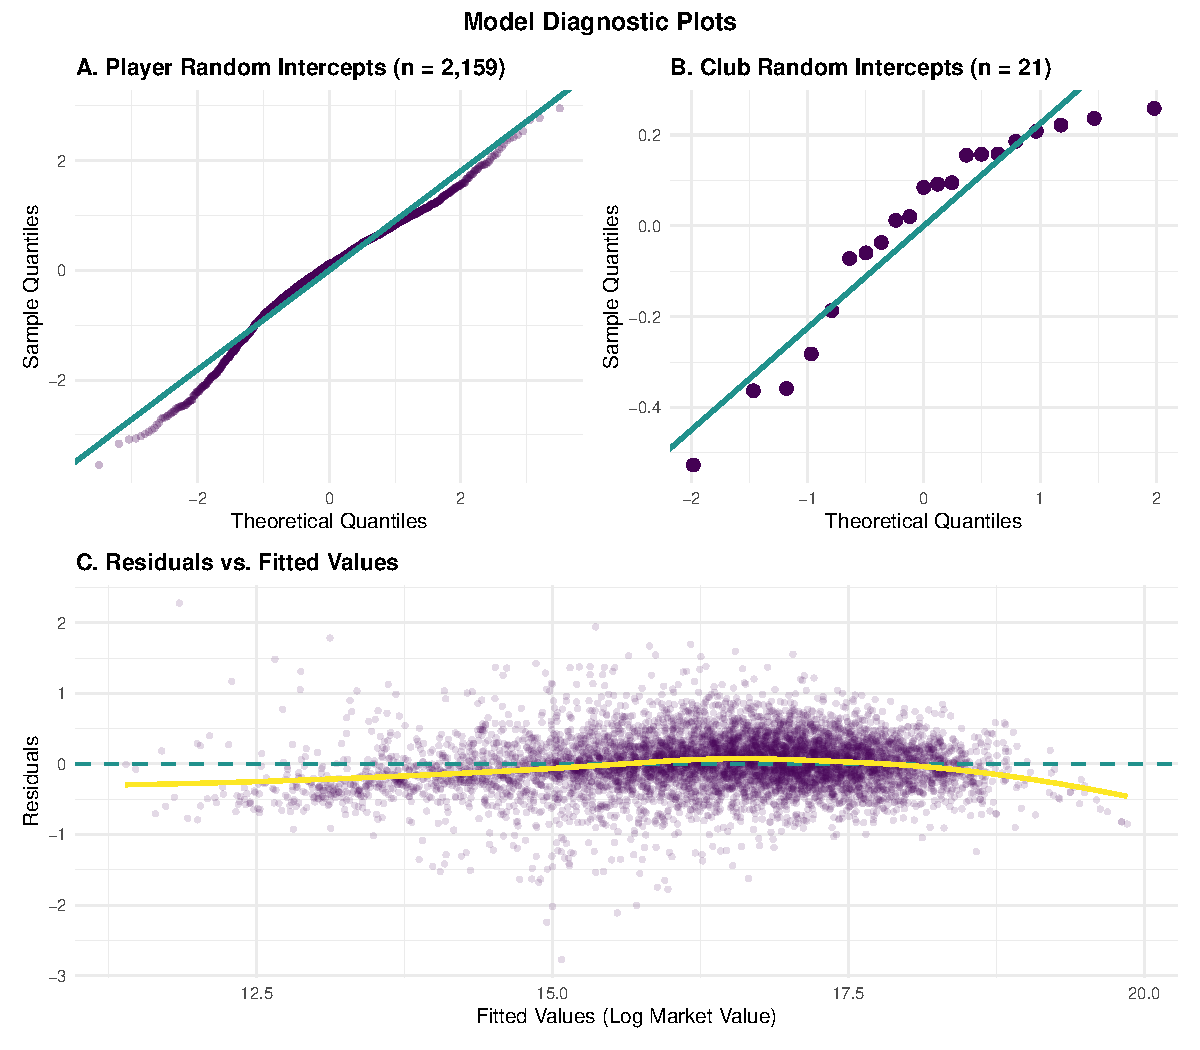
\includegraphics{Project_Paper_files/figure-pdf/unnamed-chunk-12-1.pdf}

}

\caption{Diagnostic plots: (A) Q-Q plot for player random intercepts,
(B) Q-Q plot for club random intercepts, (C) residuals versus fitted
values.}

\end{figure}%

\subsection*{Figure 7. Club Random Effects Correlation
Structure}\label{figure-7.-club-random-effects-correlation-structure}
\addcontentsline{toc}{subsection}{Figure 7. Club Random Effects
Correlation Structure}

\begin{figure}[H]

{\centering 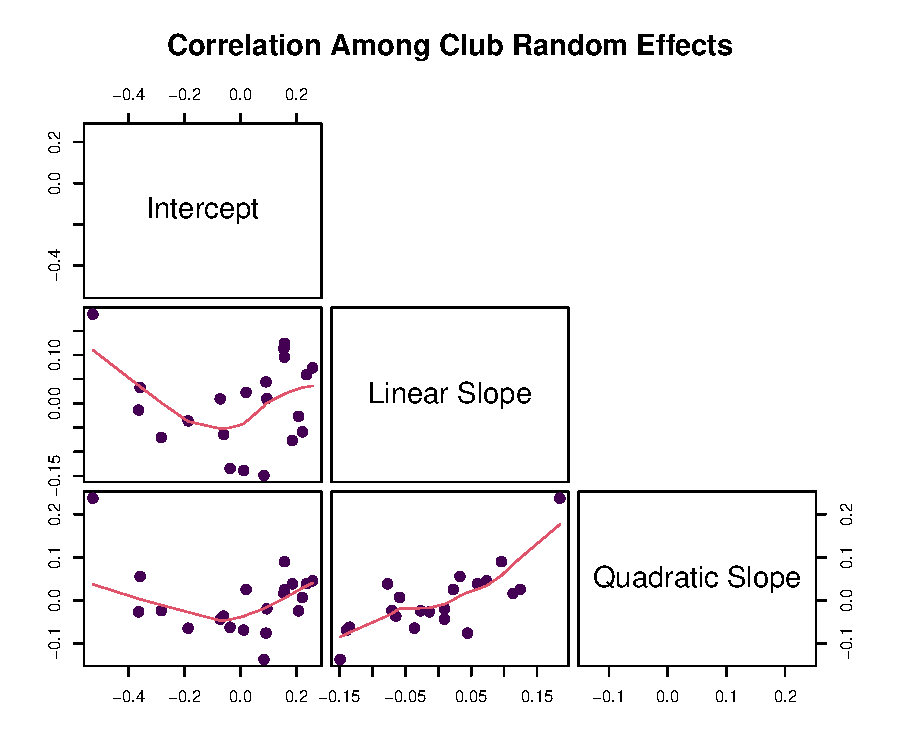
\includegraphics{Project_Paper_files/figure-pdf/unnamed-chunk-13-1.pdf}

}

\caption{Correlations among club-level random effects (intercept, linear
slope, quadratic slope).}

\end{figure}%

\newpage

\section{Appendix D}\label{appendix-d}

\subsection*{Acknowledgement of AI
Assistance}\label{acknowledgement-of-ai-assistance}
\addcontentsline{toc}{subsection}{Acknowledgement of AI Assistance}

We acknowledge the use of AI-assisted tools (GitHub Copilot and Claude)
during the preparation of this manuscript. These tools were used for:

\begin{enumerate}
\def\labelenumi{\arabic{enumi}.}
\item
  \textbf{Coding assistance}: Generating and debugging R code for data
  visualization, particularly for creating the faceted club trajectory
  plots (Figure 3) and diagnostic visualizations (Figure 6).
\item
  \textbf{Resolving convergence issues}: Troubleshooting model
  convergence problems with the cross-classified multilevel model,
  including optimizer selection (BOBYQA) and parameter constraints.
\item
  \textbf{Code documentation}: Improving comments and annotations in the
  model syntax presented in Appendix B.
\end{enumerate}

All statistical analyses, interpretations, and substantive conclusions
were developed and verified by the authors. The AI tools served as
coding assistants and did not contribute to the research design, data
collection, or theoretical framework of this study.




\end{document}
